\documentclass[../main.tex]{subfiles}

\begin{document}

\chapter{Gặp trưởng lão làng thơ Việt}

\begin{metadata}

\begin{flushright}18.9.2008\end{flushright}

Hồ Bất Khuất



\end{metadata}

\begin{multicols}{2}

Cái tên “Hữu Loan” từ lâu đã “làm tổ” trong lòng những người yêu thơ. Chỉ với bài “Màu tím hoa sim”, ông đã làm tím thi đàn Việt Nam. Đời người, đời thơ của Hữu Loan chứa đầy những điều đáng trân trọng. 
  
 
\textbf{Từ ám ảnh thuở học trò đến chuyến đi ngẫu hứng} 
  
Khi là học sinh chuyên văn của tỉnh Nghệ An, tôi chứng kiến cánh học trò chuyền tay nhau chép bài thơ “Màu tím hoa sim”. Hơn thế nữa, trong những lần đi rừng hái củi, mấy người bạn còn khe khẽ hát: “Ôi những đồi hoa sim, những đồi hoa sim tím chiều hoang biền biệt…” Tôi rất xúc động. Cái tên Hữu Loan găm vào tôi từ ngày đó.  
    
Thú thật là ngoài chuyện bài thơ hay ra, người ta còn kể nhiều chuyện khá ly kỳ về Hữu Loan. Điều đấy khiến tôi tò mò. Tôi có mong ước được gặp gỡ và trò chuyện với người “làm tím thi đàn Việt Nam”. Tôi cũng bỏ công ra sưu tầm thơ Hữu Loan, nhưng ngoài “Màu tím hoa sim” ra, tôi cũng chỉ biết thêm được “Đèo cả”. 
     
Thời gian cứ thế trôi, tôi tốt nghiệp đại học rồi đi làm báo. Công việc và chuyện “cơm áo gạo tiền” cuốn đi mải miết. Bạn bè cùng học, cùng uống rượu thành nhà văn, nhà thơ; họ in sách tặng tôi xếp đầy cả tủ. Bản thân tôi cũng bỏ tiền mua những tập không được tặng, nhưng tôi tìm mãi vẫn không thấy tập thơ nào của Hữu Loan. Tôi vẫn khắc khoải, mong ngóng một điều gì đấy. 
\textbf{   } 
... Vào những năm tám mươi của thế kỷ trước, trong một lần đi công tác tại Thanh Hoá, khi xe của chúng tôi đi qua một làng quê, người ngồi bên cạnh tôi thì thầm: "Hình như nhà thơ Hữu Loan kìa". Theo tay anh chỉ, tôi thấy một người đàn ông trên 60 tuổi đẩy một chiếc xe thồ đầy đá. Chiếc U-uát chạy nhanh quá, tôi không nhìn rõ mặt người đẩy xe, nhưng thấy dáng ông đi tự tin và vững chãi. Tuy nhiên, hình ảnh ấy có vẻ không phù hợp với một thi sĩ. Chắc có điều gì uẩn khúc ở đây? Tôi mong được một lần gặp Hữu Loan. 
    
Mãi đến bây giờ tôi mới có dịp thực hiện mơ ước từ ngày bé của mình. Vào một ngày đẹp trời, có người rủ tôi đi thăm nhà thơ Hữu Loan. Tôi mừng húm vì nghĩ rằng, người này có mối quan hệ thân thiết với nhà thơ nổi tiếng. Nhưng hoá ra không phải vậy. Anh cũng chỉ là người mến mộ nhà thơ và biết mỗi địa chỉ. Nhưng khi đã muốn thì có thể tìm… 
       
Cách thành phố Thanh Hoá khoảng 26 km, trên quốc lộ 1A (hướng Hà Nội – Vinh), có biển chỉ dẫn "Nga Sơn" đi về phía biển. Theo con đường này đi được chừng 2 km, chúng tôi hỏi hai cô gái đi xe máy cùng chiều. Thật may, hai cô này quê ở Nga Lĩnh và biết nhà của thi sĩ Hữu Loan. Hai cô tình nguyện dẫn đường cho chúng tôi. Trước khi về nhà mình, các cô nói: "Đi theo đường này khoảng vài trăm mét, thấy cái nhà 2 tầng, ông Hữu Loan ở đó.” 
 \begin{blockquote}
Nhà thơ Hữu Loan tên thật là Nguyễn Hữu Loan, sinh ngày 02/4/ 1916 tại xã Nga Lĩnh, huyện Nga Sơn, tỉnh Thanh Hoá. Ông tham gia hoạt động cách mạng từ năm 1936, đã từng giữ chức Phó Chủ tịch Uỷ ban Khởi nghĩa Nga Sơn, Uỷ viên Văn hoá trong Uỷ ban Lâm thời tỉnh Thanh Hoá. Trong kháng chiến chống Pháp, ông là chiến sĩ một đơn vị ở Liên khu 4, chủ bút báo \textit{Chiến sĩ}. Sau năm 1954, ông làm ở báo \textit{Văn nghệ}, Hội Nhà văn Việt Nam. Sau đó, ông trở về quê làm ăn sinh sống và nuôi dạy con cái. \end{blockquote}
 Tuy đã tìm được gần đến nơi, nhưng trong tôi cảm xúc lẫn lộn. Tôi chưa tưởng tượng được nhà thơ Hữu Loan hơn 90 tuổi, ở trong một ngôi nhà tầng sang trọng, lên xuống cầu thang như thế nào. Và nữa, ông có thể không có nhà. Nếu ở nhà, ông có thể không tiếp chúng tôi, vì trước khi đến đây chúng tôi chẳng liên hệ, chẳng có thông tin gì cả, ngoại trừ cái địa chỉ: thôn Vân Hoàn, xã Nga Lĩnh, huyện Nga Sơn. 
    
 \begin{figure}
	\centering
	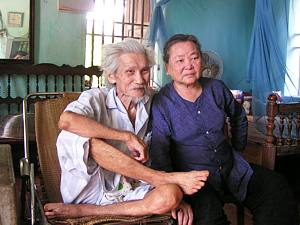
\includegraphics[width=\textwidth]{../img/tho180908_1.jpg}
	\caption{Vợ chồng nhà thơ Hữu Loan }
\end{figure}
 Nhưng mọi sự không như tôi tưởng. Cái nhà 2 tầng hoá ra không phải của gia đình Hữu Loan, mà chỉ là một cái nhà nổi bật ở gần đó. Nhà thơ Hữu Loan ở trong một ngôi nhà cấp 4 chật chội, cũ kỹ; bù lại, có mảnh vườn khá rộng, có dừa vươn mình soi bóng, giàn mướp nở hoa vàng rực rỡ và một ao cá nhỏ xinh.  
     
 Tôi hồi hộp bước vào và thấy một ông già tóc bạc trắng. Đấy là nhà thơ Hữu Loan; ngồi cạnh một phụ nữ đã cao tuổi nhưng trông vẫn khoẻ mạnh, là vợ nhà thơ. Thấy chúng tôi vào, vợ chồng nhà thơ không ngạc nhiên, không tỏ ra vui mừng, đon đả, nhưng thân mật. Ông bà không hỏi chúng tôi là ai, đến đây làm gì, chỉ mời nước và quay quạt về hướng chúng tôi. Có lẽ những cuộc viếng thăm của các nhà văn, nhà báo, hay đơn giản chỉ là của những người yêu thơ đã trở nên quen thuộc với vợ chồng nhà thơ Hữu Loan. 
  
 
\textbf{Mối tình thánh thiện, đau thương và tuyệt tác thơ "Màu tím hoa sim”}    \textbf{   } 
\begin{blockquote}
Gia đình ông Lê Đỗ Kỳ là một gia đình trí thức cách mạng. Ông là kỹ sư canh nông, đã từng giữ chức Tổng Thanh tra Canh nông Đông Dương. Vợ là con một nhà khoa bảng đất Thanh Hoá. Sau Cách mạng tháng Tám năm 1945, ông Kỳ là đại biểu Quốc hội khoá đầu tiên. Vợ ông trở thành cán bộ của Hội Phụ nữ. Ba người con trai đầu của ông đi bộ đội. Người con cả là Lê Đỗ Khôi, hy sinh trên đồi Him Lam ngay trước giờ chiến thắng Điện Biên. Người con thứ hai là Lê Đỗ Nguyên, chính là Trung tướng Phạm Hồng Cư. Người con thứ ba Lê Đỗ An chính là Nguyễn Tiên Phong, nguyên bí thư Trung ương Đoàn, nguyên Phó Ban Dân vận Trung ương. Người con thứ tư là Lê Đỗ Thị Ninh, vợ của nhà thơ Hữu Loan, nhân vật chính của bài thơ "Màu tím hoa sim". \end{blockquote}
 Chàng gia sư tài hoa và cô học trò xinh đẹp đã cảm mến nhau ngay từ khi chàng đặt chân đến nhà nàng. Chẳng thế mà nàng tự tay giặt là quần áo cho chàng, mặc dù trong gia đình có hàng chục người được thuê để lo việc nhà. Dù đã thầm yêu nàng tha thiết, nhưng vì "không môn đăng hộ đối" nên chàng chẳng dám ngỏ lời. Nhưng người quyết liệt lại là nàng. Nàng chủ động bắt chuyện với chàng, đưa chàng đi dạo ở những dải đồi nở đầy hoa sim tím. Rồi nữa, áo nàng mặc tím màu hoa sim. Trong những ngày chàng lãnh đạo khởi nghĩa ở địa phương thì nàng cũng tham gia công tác quần chúng. Khi chàng làm việc ở Uỷ ban Lâm thời tỉnh Thanh Hoá thì nàng là một trong những người tích cực vận động nhà giàu tham gia hưởng ứng “Tuần lễ vàng”. Cái không khí phơi phới, lạc quan của những đầu cách mạng thành công đã khiến cho tình yêu của họ vốn đã lãng mạn, càng thêm lãng mạn. 
    
Trước một tình yêu chân thành, mãnh liệt, tinh tế và quả cảm của người con gái đẹp; thông minh, đa cảm, tài hoa như Hữu Loan không thể không tiếp nhận. Đây là hạnh phúc mà không phải ai cũng có được: Yêu và được con gái của nhà giàu yêu, rồi chính bố mẹ cô ta đứng ra làm đám cưới. 
     
Hữu Loan cưới vợ trong một lần về phép ngắn ngủi, rồi lại ra đi, mải miết theo đoàn quân trong cuộc trường chinh chống Pháp. Nhưng cuộc đời thật khó lường, “không chết người trai khói lửa, mà chết người con gái hậu phương”. Vợ Hữu Loan chết khi mới 17 tuổi, số ngày sống với chồng chỉ tính trên đầu ngón tay.  
     
Nhận được tin vợ chết, Hữu Loan từ đơn vị trở về, thấy mẹ ngồi bên nấm mồ, bình hoa ngày cưới đã thành bình hương. Trong tim Hữu Loan - người lính, người tình, người chồng, người con dâng lên những đợt sóng trào. Tình cảm thiết tha, mãnh liệt và nỗi đau sâu thẳm đã sản sinh ra bài thơ "Màu tím hoa sim". Tất cả những tình tiết, sự kiện, con người trong bài thơ đều là thật. Có lẽ đây chính là nguyên nhân để bài thơ trở nên bất tử.  
     \begin{blockquote}
Cho đến lúc này, người ta vẫn chưa biết nhà thơ Hữu Loan đã viết tất cả bao nhiêu bài thơ. Nhà thơ, nhà nghiên cứu Vũ Quần Phương thì khẳng định: Hữu Loan viết tất cả 24 bài. Một số nhà nghiên cứu khác nói ông viết được khoảng 40 bài. Một người con trai của ông đang tìm tòi, sưu tập bản thảo viết tay tất cả những bài thơ của ông. Anh chưa chính thức công bố vì chưa hoàn chỉnh, nhưng theo anh, toàn bộ sáng tác của bố anh không quá 60 bài thơ. \end{blockquote}
 Cả cuộc đời dài gần trăm năm của mình, Hữu Loan làm thơ không nhiều, không in tập lớn, tập bé; nhưng chỉ cần với một “Màu tím hoa sim”, ông đã nhuộm tím thi đàn Việt Nam. Cái màu tím bình dị của một loài cây mọc lúp xúp ở đồi núi Việt Nam đã trở thành một trong những biểu tượng đẹp của thơ ca. 
 
 
\textbf{Chuyện đời mộc mạc} 
    
 \begin{figure}
	\centering
	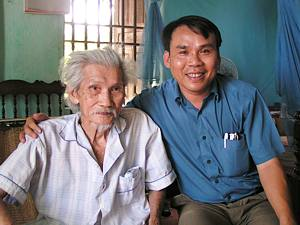
\includegraphics[width=\textwidth]{../img/tho180908_2.jpg}
	\caption{Nhà thơ Hữu Loan và tác giả Hồ Bất Khuất}
\end{figure}
 Người ta đã viết nhiều về Hữu Loan và dành cho ông những lời lẽ tốt đẹp nhất. Tôi không muốn làm cái chuyện ấy nữa, chỉ ngồi ngắm nhìn, hỏi chuyện, nghe ông nói, đọc thơ. Ở tuổi 93, vẫn với ánh mắt cười rất hóm, nhà thơ Hữu Loan chậm rãi kể cho chúng tôi nghe về cuộc đời mình.  
 
“Tôi sinh ra trong một gia đình nghèo, nhưng rất sùng bái chuyện học hành. Ngày bé, tôi tự học là chính. Năm 1938, tôi ra Hà Nội thi, gặp gỡ Nguyễn Đình Thi từ dạo đó. Trở về Thanh Hoá, tôi làm gia sư, vừa để kiếm sống, vừa để học thêm, vừa có điều kiện tham gia cách mạng. 
    
Khi tôi đến dạy học ở nhà một người quyền quý, cô con gái của gia chủ nhìn tôi bằng ánh mắt rất lạ. Tôi bị ánh mắt và gương mặt đẹp thánh thiện ám ảnh, nhưng không dám nghĩ tới chuyện xa hơn. 
    
Nhưng thật may mắn, tôi là chàng trai nghèo nhưng lại được cô học trò xinh đẹp là con của một người sang trọng và giàu có yêu. Chúng tôi đã được yêu nhau và hạnh phúc, tuy rất ngắn ngủi. Sau khi Lê Đỗ Thị Ninh chết, tôi nghĩ là mình chẳng bao giờ lấy vợ nữa, ấy thế mà…” 
    
Ông dừng lời và đưa mắt tình tứ nhìn vợ là bà Phạm Thị Nhu ngồi bên cạnh. Đây là người phụ nữ gắn bó với ông suốt cả cuộc đời, sinh cho ông 10 người con. Bà Nhu nói: 
 
“Tôi yêu ông này vì ngày ấy hay ra nghe trộm ông giảng Truyện Kiều cho học sinh. Trọng tài rồi mê người lúc nào không rõ nữa. Dù ông ấy hơn tôi những 20 tuổi, nhưng tôi vẫn mê ông và khiến ông bỏ ý định không lấy vợ nữa. Ông ấy lại còn viết bài thơ ‘Hoa lúa’ nịnh tôi nữa chứ.” 
\textit{    } 
Nhà thơ Hữu Loan nhìn vào xa xăm rồi tiếp lời vợ: 
  
"Màu tím hoa sim" là khóc người vợ đã chết, còn "Hoa lúa" là bài thơ viết cho bà đang ngồi đây!” 
 
“Ông ấy nhớ toàn bộ bài này đấy, bảo ông ấy đọc cho mà nghe!” - Vợ thi sĩ thì thầm, nhưng cũng đủ cho tất cả mọi người trong căn nhà nghe rõ.  
\textit{  }    
Bằng một chất giọng hơi khàn nhưng vẫn ấm, nhà thơ Hữu Loan đọc bài "Hoa lúa". Bài thơ khá dài, nhưng ông đọc thong thả, khi thì nhìn ra khoảng sân có dàn mướt đơm hoa, kết trái; khi thì nhìn về phía người đàn bà đã gắn bó cùng ông hơn nửa thế kỷ. Vợ ông ngồi lim dim, mãn nguyện. Có hạnh phúc nào hơn khi người mình say mê trở thành chồng mình, làm thơ tình tặng mình, thỉnh thoảng lại dồn hết tâm trí vào đó và tha thiết đọc lên. 
\textbf{   } 
 
\textbf{Sự bình dị của nhân cách lớn} 
  
Thật khó mà tưởng tượng hết những khó khăn mà Hữu Loan vượt qua để duy trì cái gia đình có 12 miệng ăn giữa vùng quê nghèo khó trong những năm chiến tranh ác liệt. Hơn nữa, nhiều người trong bộ máy chính quyền địa phương lúc ấy không hiểu ông, còn gây thêm cho ông những khó khăn như tịch thu xe đạp của ông với lý do… phụ tùng không đồng bộ; xúi giục những người khai thác đá không bán cho ông. 
\textbf{   } 
Bằng nghị lực và sự dẻo dai hiếm có cả về tinh thần lẫn thể chất, Hữu Loan đã vượt qua tất cả mọi thử thách, tai ương. Ông đã sống, làm việc bền bỉ, trung thực, ngay thẳng để vợ con yên bình, vững tâm mà sống, mà lớn. Người ta không bán đá cho ông thì tự tay ông khai thác và chở đi bán. Một mình ông gần như đã san bằng một ngọn núi. Ông cũng đã trở thành “chuyên gia” mò cua, bắt ốc ở nơi những cây cói mọc lên để thành chiếu Nga Sơn nổi tiếng. Có lẽ trước khi khăn gói rời Hà Nội, ông đã lường trước mọi khó khăn nên không điều gì có thể làm ông gục ngã. 
      
Nhưng theo ông, tình yêu và trách nhiệm với vợ con mới là nguồn sức mạnh lớn lao giúp ông đứng vững giữa cuộc đời. Ông bảo: “Tôi là người ương bướng, hay cãi. Ở lại làm trong cơ quan, đoàn thể, khó mà dung hoà với mọi người được. Nếu vậy thì làm sao nuôi nổi đàn con? Nghĩ vậy, tôi thấy về với vợ con là tốt nhất.” 
     
10 người con của ông đã trưởng thành, có người là giáo viên, có người là kiến trúc sư, có người là nông dân… Bây giờ mọi thứ qua rồi nên ông nhớ lại mọi thứ, nhẹ nhàng, thanh thản. Hữu Loan cho biết, ông vẫn làm thơ nhưng rất ít, và hầu như không in ở đâu. Phần lớn thời gian ông suy ngẫm để tìm ra vế đối của những câu thách đố nổi tiếng kiểu “Da trắng vỗ bì bạch”. Ông cho biết đã đối khá chỉnh nhiều vế đối của Hồ Xuân Hương, Đoàn Thị Điểm.  
     
Cách đây mấy năm, Công ty Vitek đặt vấn đề xin được chuyển nhượng tác quyền bài thơ “Màu tím hoa sim” 100 triệu đồng. Lúc đầu ông không chịu với lý do “thơ tôi làm ra không phải để bán”, nhưng khi thấy có những người con vẫn còn khó khăn về vật chất, ông đã đồng ý. Sau khi nộp thuế 10 triệu đồng, ông mang 60 triệu chia cho các con, chỉ giữ lại 30 triệu cho tuổi già. 
     
Hai vợ chồng nhà thơ Hữu Loan sống trong ngôi nhà nhỏ bé, ấm cúng, xung quanh là vườn cây xanh tốt; không xe hơi nhà lầu, không hội họp, phê bình, kiểm điểm, không đọc báo cáo… Hàng ngày ông trò chuyện với vợ, đọc thơ, chơi với các cháu và tiếp khách. Người làm tím thi đàn Việt Nam sống bình dị giữa làng quê của mình với đôi mắt cười rất hóm. 
 
© 2008 talawas 
\end{multicols}
\end{document}